\documentclass[10pt]{scrartcl} 

\usepackage[a4paper,left=1.5cm,right=1.5cm,top=2cm,bottom=2cm,bindingoffset=5mm]{geometry}

%% allgemeine Imports, die nicht mehr erforderlich sind, da ich mit lulatex kompiliere
% \usepackage[utf8x]{inputenc} % Zeichenkodierung
% \usepackage[ngerman]{babel}  % u.a. Silbentrennung
% \usepackage[T1]{fontenc}

%\usepackage{floatflt} 
%\usepackage{times}

\usepackage{amsmath} %Bei Bedarf: Formeln
\usepackage{graphicx}   % Bilder
\graphicspath{{./image/}{./plantuml/}{./}}
%\begin{figure}[htbp] 
%	\centering
%	\includegraphics[width=3cm]{JavaSpringInitializr.png}
%	\caption{Logo}
%	\label{fig:Bild1}
%\end{figure}

\usepackage{tabularx}
\usepackage{booktabs}
\usepackage{calc} % Zur Berechnung von \ht und \structbox scheinbar nötig

\usepackage{wrapfig}
%\begin{wrapfigure}{l}{0.25\textwidth}
%	\centering
%	\includegraphics[width=0.25\textwidth]{contour}
%\end{wrapfigure}

\usepackage{lastpage} %Letzte Seitenzahl anzeigen
\usepackage{hyperref}
\usepackage{cclicenses}

%\usepackage{blindtext}  %% Zum Debugging: Blindtext einfügen

%%% zur Darstellung von Quellcode
\usepackage{listings}
\usepackage{color}
\usepackage{xcolor}

%%% Für individuelle Kopfzeilen
% https://esc-now.de/_/latex-individuelle-kopf--und-fusszeilen/?lang=en
%%%%%%%%%%%%%%%%%%%%%%%%%%%
\usepackage[headsepline=0.5pt,footsepline=0.5pt,plainheadsepline=true, plainfootsepline=true,headwidth=(\the\textwidth), footwidth=(\the\textwidth)]{scrlayer-scrpage}

% Alle Inhalte löschen.
\clearpairofpagestyles

%\renewcommand{\familydefault}{\sfdefault}

% Schriftformatierung zurücksetzen.
\setkomafont{pageheadfoot}{}
\setkomafont{title}{\bfseries}

% Linien einfärben.
\addtokomafont{headsepline}{\color{gray}}
\addtokomafont{footsepline}{\color{gray}}

% Statische Inhalte.
\ihead{\thetitle}
%\chead{Mitte oben}
\ohead{
	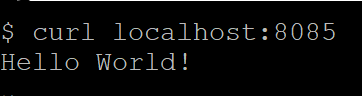
\includegraphics[height=1cm]{logo}	
}


% Unterschiedliche Inhalte für gerade/ungerade.
\ifoot*{\href{https://creativecommons.org/licenses/by/4.0/}{\ccby CC BY 4.0}, Hannes Stein  }
\cfoot*{\today}
\ofoot*{\pagemark}
\renewcommand*{\pagemark}{{\usekomafont{pagenumber}{Seite \thepage\ von \pageref*{LastPage}}}}


%\usepackage{showframe} % for debug information
\usepackage{titling}
\pretitle{
	
	\begin{tabular}[b]{p{11cm} p{5cm}}
		\bfseries
		\LARGE
		\selectfont
	}
	\posttitle{
		& 	
		\raisebox{-\height}{
			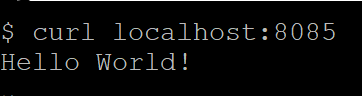
\includegraphics[width=4.5cm]{logo}
		}
	\end{tabular}
}
%\preauthor{}\postauthor{}
\predate{}\date{}\postdate{}


%%%%%%%%%%%%%%%%%%%%%%%%%


%%% zur Darstellung von Quellcode
\definecolor{dkgreen}{rgb}{0,0.6,0}
\definecolor{gray}{rgb}{0.5,0.5,0.5}
\definecolor{lightgray}{rgb}{0.83, 0.83, 0.83}
\definecolor{mauve}{rgb}{0.58,0,0.82}

\lstset{
	frame=tb,	
	aboveskip=3mm,
	belowskip=3mm,
	columns=fixed,
	basicstyle={\small\ttfamily},
	numbers=left,
	numberstyle=\tiny\color{gray},
	firstnumber=last,
	keywordstyle=\color{blue},
	commentstyle=\color{dkgreen},
	stringstyle=\color{mauve},
	breaklines=true,
	breakatwhitespace=true,
	tabsize=3,
	includerangemarker=true,
	showtabs=false,
	showspaces=false
}

\lstdefinestyle{java}{
	language=Java,
	numbers=left, stepnumber=1, numberstyle=\tiny, numbersep=10pt}
\lstdefinestyle{bashquery}{
	language=bash,
	numbers=left,
	stepnumber=1,
	numberstyle=\tiny,
	numbersep=10pt}
\lstdefinestyle{response}{
	frame=trbl,
	aboveskip=0mm,
	belowskip=3mm,
	basicstyle={\scriptsize\ttfamily},
	frame=shadowbox, 
	rulecolor=\color{lightgray},
	rulesepcolor=\color{lightgray},
	numbers=none
}

\lstdefinestyle{nonumbers}{
	numbers=none
}

\lstdefinestyle{plantuml}{
	numbers=left, stepnumber=1, numberstyle=\tiny, numbersep=10pt,
	morekeywords=[1]{actor, usecase, rectangle, as},
	morekeywords=[2]{skinparam, ArrowColor, BorderColor, BackgroundColor},
	morekeywords=[3]{DefaultFontName},
	morekeywords=[4]{whitesmoke, DarkSlateBlue, LightYellow},
	morekeywords=[5]{note, top, on, link, end, left to right, direction, up, down},
	otherkeywords={ :,  .., .,  -, --, ->, -->, -|>, --|>, <-, <--, <|-, <|--, <., <.., <|., <|.., \\n, \{, \}} ,
	morecomment=[l]{'}
}

\lstdefinestyle{powershell}{
	alsodigit = {-},
	morekeywords=[1] = {Get-AzureSubscription,Get-Host,anything}
}

%\hypersetup{
%	pdftitle    = { hihihi },
%	pdfsubject  = {Um was geht es },
%	pdfauthor   = {Autor bzw. Autoren},
%	pdfkeywords = {Stichwort1, Stichwort2 ...} ,
%	baseurl = {http://www.csbme.de},
%	pdfdisplaydoctitle = true
%}


\title{Hello SpringBoot - ein erstes Projekt}
%\author{Hannes Stein}





\begin{document}
	\setlength{\droptitle}{-40pt} % lower the title
	\maketitle
	%	\begin{abstract}
	%	Wie interagiert ein (Software-)System mit dem Benutzer?
	%	\end{abstract}
	
	
	
	%\pagenumbering{roman}\setcounter{page}{1}
	% \tableofcontents
	% \listoffigures
	% \listoftables
	
	
	
	\pagenumbering{arabic}\setcounter{page}{1}
	



\begin{abstract}
 Mit einem installierten SpringBoot-Framework  ein ''HelloWorld''-Projekt starten.	
\end{abstract}

\section{Ein erstes Projekt erstellen}

\begin{tabularx}{\textwidth}{Xc}
	
	\addlinespace
	Nach der Installation von \textit{NB SpringBoot} findet sich unter File / New Project eine neue Rubrik
	&
	\raisebox{\ht\strutbox-\height}{
		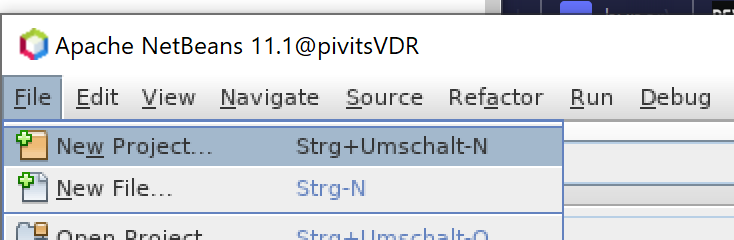
\includegraphics[width=5.5cm]{FirstProject/00_NewProject}
	}
	\tabularnewline 
	 \hline
\addlinespace
"Java with Maven" / "Spring Boot Initializr Project"
&
\raisebox{\ht\strutbox-\height}{
	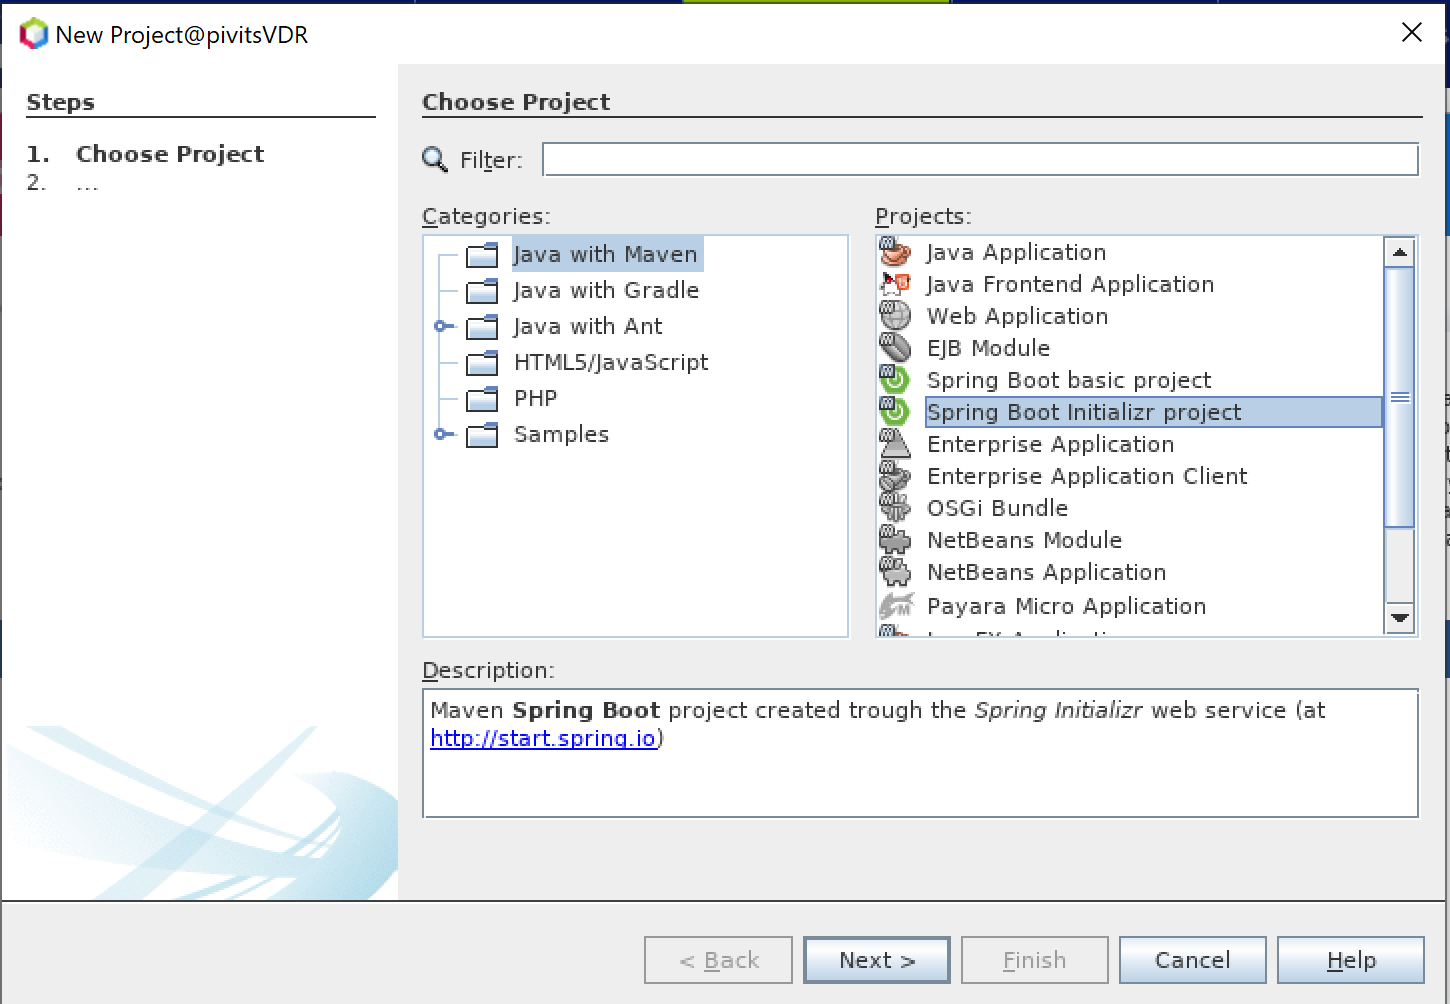
\includegraphics[width=5.5cm]{FirstProject/01_ChooseSpringBootInitializr}
	}
	\tabularnewline 
	 \hline
\addlinespace
Im Folgenden werden müssen eine Reihe von Projektdaten angegeben werden.
Wer nicht Netbeans nutzt kann sein Projekt auch unter \linebreak
\url{https://start.spring.io/} mit einer identischen Maske erstellen.
&
\raisebox{\ht\strutbox-\height}{
	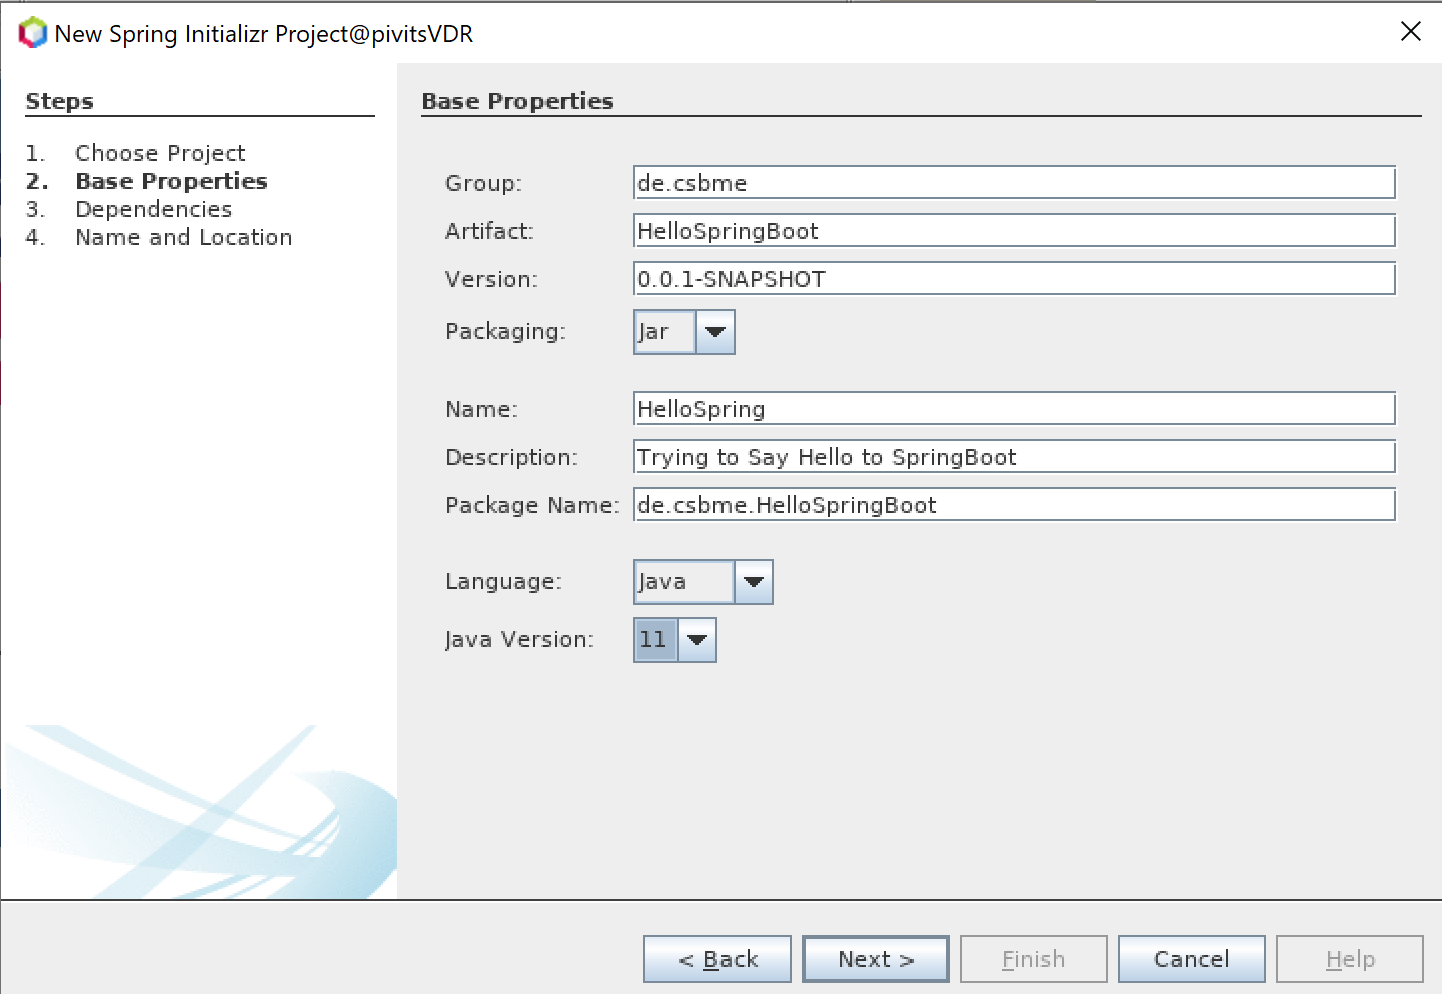
\includegraphics[width=5.5cm]{FirstProject/02_BaseProperty}
	}
\tabularnewline  \hline
\addlinespace
Group: \linebreak
Artifact: \linebreak
Version:\linebreak
&
\raisebox{\ht\strutbox-\height}{
	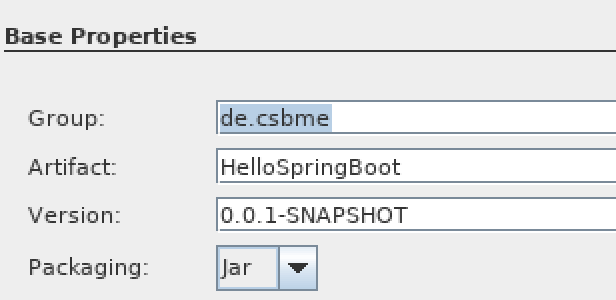
\includegraphics[width=5.5cm]{FirstProject/02_BaseProperty_Group}
}
\tabularnewline  \hline
\addlinespace
JAR: Ein mit Maven oder per Konsole ausführbares JAR-Archiv (auswählen)\linebreak
WAR: Ein Java EE-Container, der z.B. mit Tomcat genutzt wird\linebreak
Hintergrund z.B.: \url{https://www.baeldung.com/java-jar-war-packaging}
&
\raisebox{\ht\strutbox-\height}{
	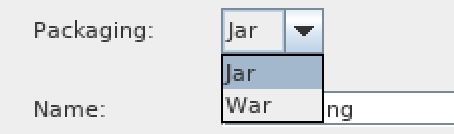
\includegraphics[width=5.5cm]{FirstProject/02_BaseProperty_Packaging}
}
\tabularnewline  \hline
\addlinespace
Name und Package Name sollten sich automatisch angepasst haben - eine Beschreibung kann noch ergänzt werden.
&
\raisebox{\ht\strutbox-\height}{
	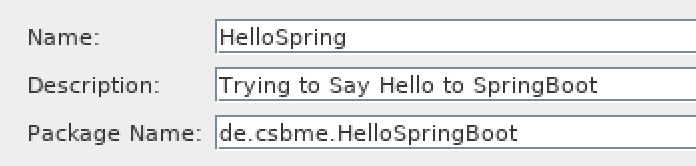
\includegraphics[width=5.5cm]{FirstProject/02_BaseProperty_Name}
}


\end{tabularx}

\begin{tabularx}{\textwidth}{Xc}
	 \hline
\addlinespace
Es stehen prinzipiell verschiedene JVM-Sprachen zur Auswahl&
\raisebox{\ht\strutbox-\height}{
	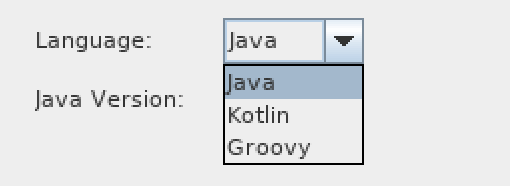
\includegraphics[width=5.5cm]{FirstProject/02_BaseProperty_Language}
}
\tabularnewline  \hline
\addlinespace
Theoretisch ist SpringBoot 2 mit Java 8 möglich - sinnvoll ist es jetzt die aktuelle JDK11 LTS zu verwenden.&
\raisebox{\ht\strutbox-\height}{
	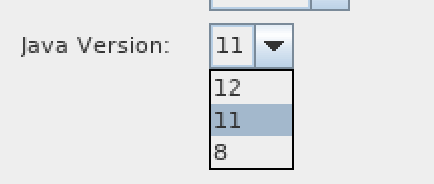
\includegraphics[width=5.5cm]{FirstProject/02_BaseProperty_JavaVersion}
}

\tabularnewline  \hline
\addlinespace
Das Startprojekt soll als einzige Abhängigkeit "Spring Web" erhalten.&
\raisebox{\ht\strutbox-\height}{
	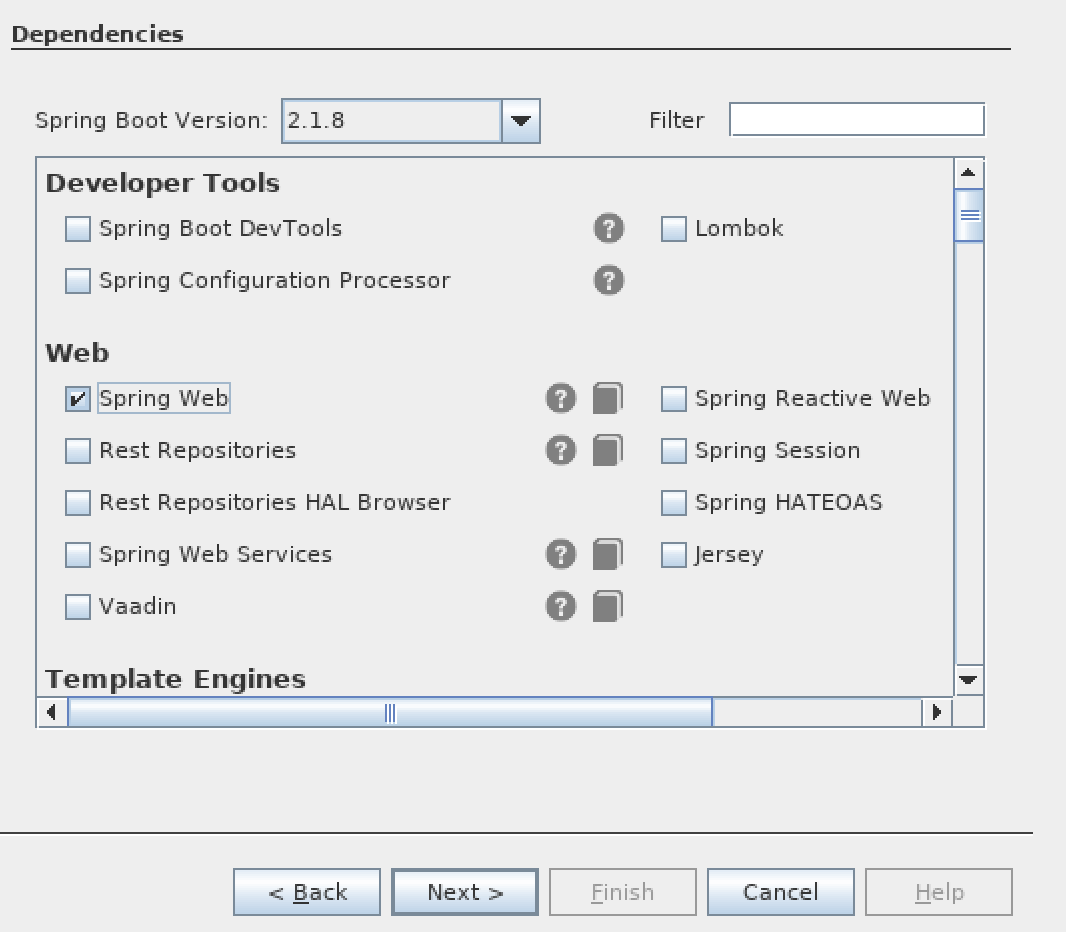
\includegraphics[width=5.5cm]{FirstProject/03_Dependencies_Web}
}
\tabularnewline  \hline
\addlinespace
Hier einfach weiterklicken oder Namen anpassen...&
\raisebox{\ht\strutbox-\height}{
	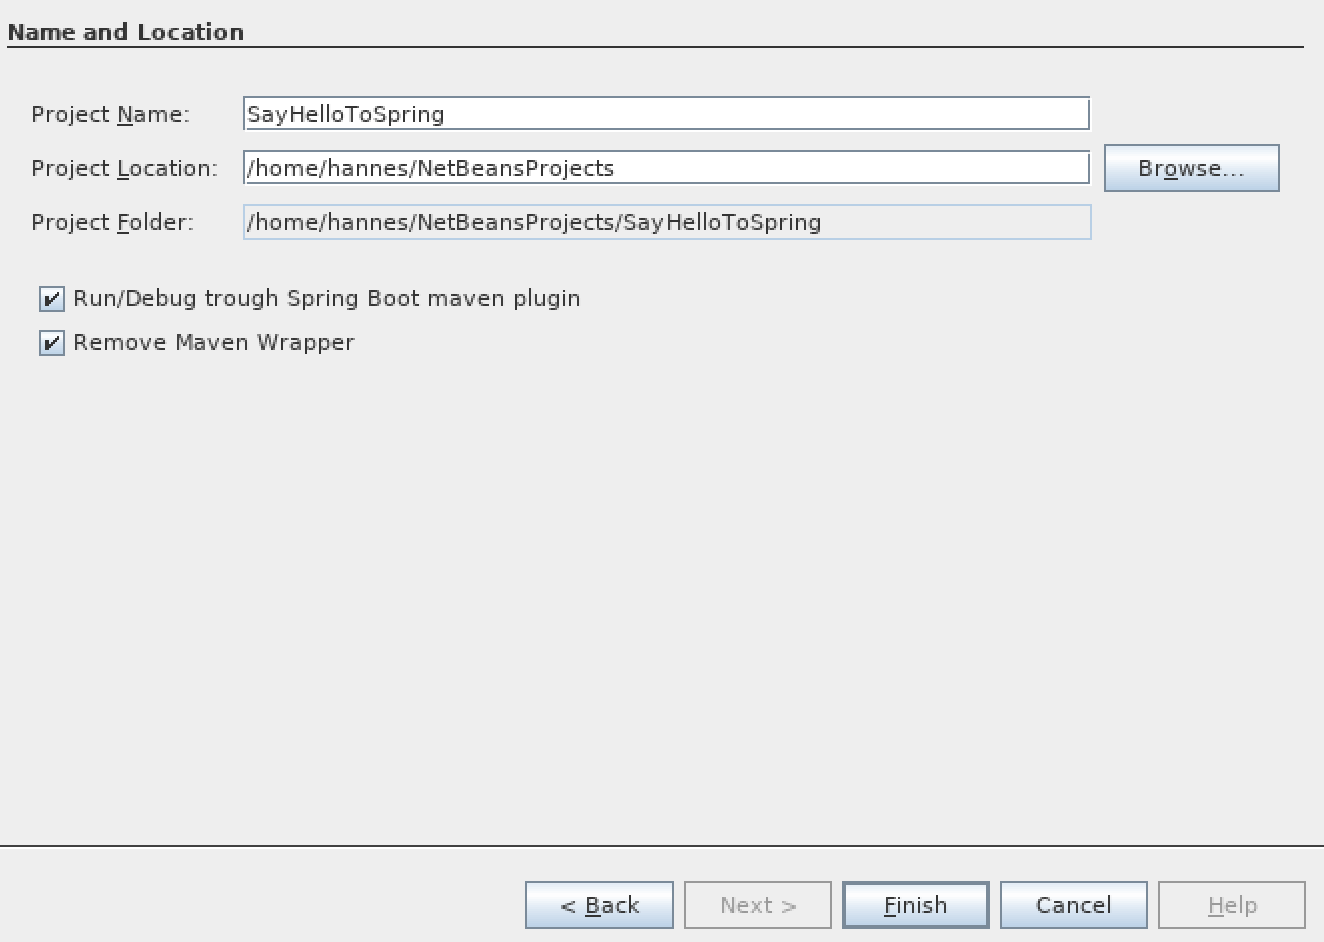
\includegraphics[width=5.5cm]{FirstProject/04_NameAndLocation}
}
\tabularnewline  \hline
\addlinespace
Es müssen erst allerlei Abhängigkeiten geladen werden, was man unten am Progressbar sieht&
\raisebox{\ht\strutbox-\height}{
	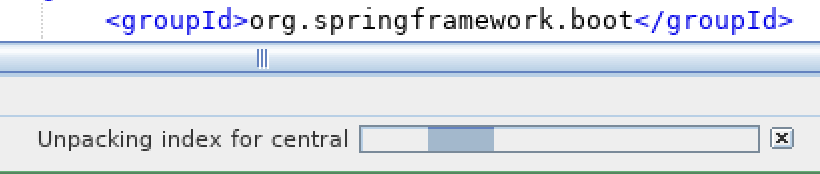
\includegraphics[width=5.5cm]{FirstProject/05_ResolveProblems_02}
}
\tabularnewline  \hline
\addlinespace
Wenn das Projekt jetzt startet holt er die Dateien...&
\raisebox{\ht\strutbox-\height}{
	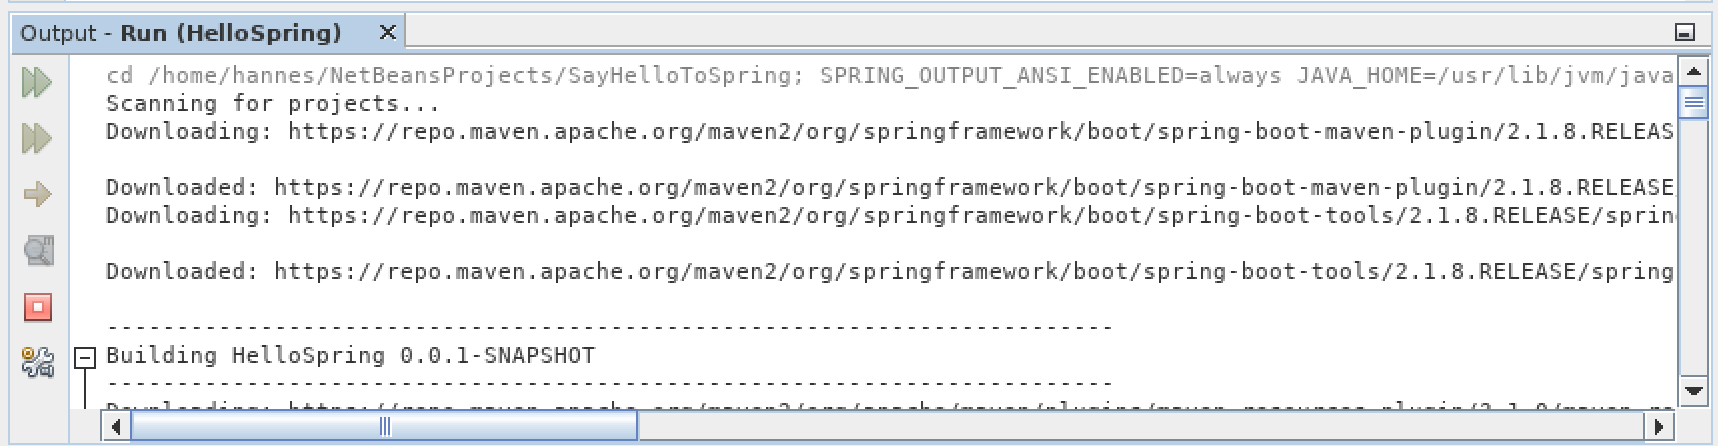
\includegraphics[width=5.5cm]{FirstProject/06_output_01}
}
\tabularnewline  \hline
\addlinespace
Zeigt ein bisschen ASCII-Art...&
\raisebox{\ht\strutbox-\height}{
	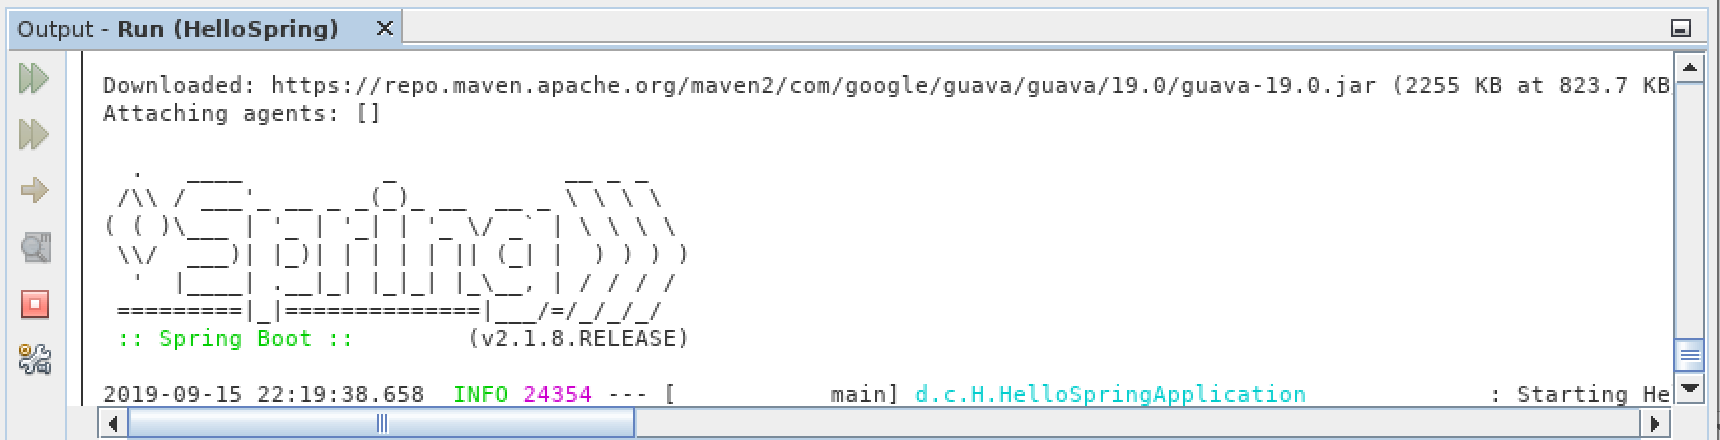
\includegraphics[width=5.5cm]{FirstProject/06_output_02}
}
\tabularnewline  \hline
\addlinespace
Und ist fertig...&
\raisebox{\ht\strutbox-\height}{
	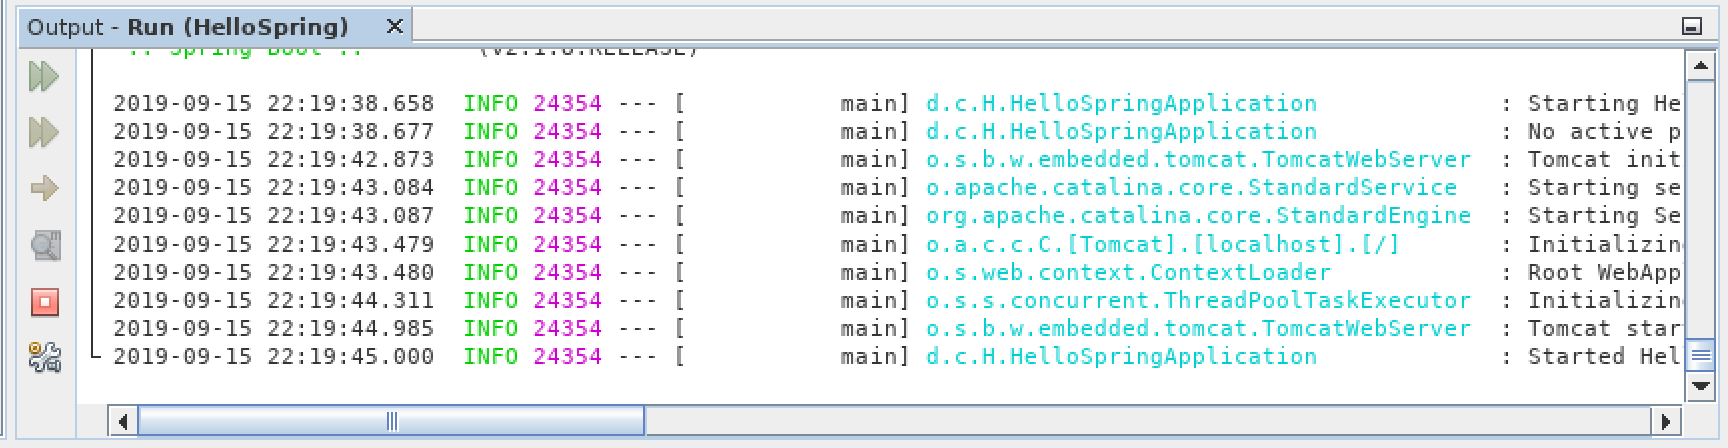
\includegraphics[width=5.5cm]{FirstProject/06_output_03}
}


\end{tabularx}

\section{Was wurde erstellt?} 

Im Wesentlichen wurden zwei Dateien erstellt: eine Application-Class (HelloSpringApplication.java) und eine Konfigurations-Datei (pom.xml). In Netbeans kann man entweder über den Projects oder den Files-Tab navigieren, um sie zu finden:

\begin{tabularx}{\textwidth}{XX}
	\hline
\raisebox{\ht\strutbox-\height}{
	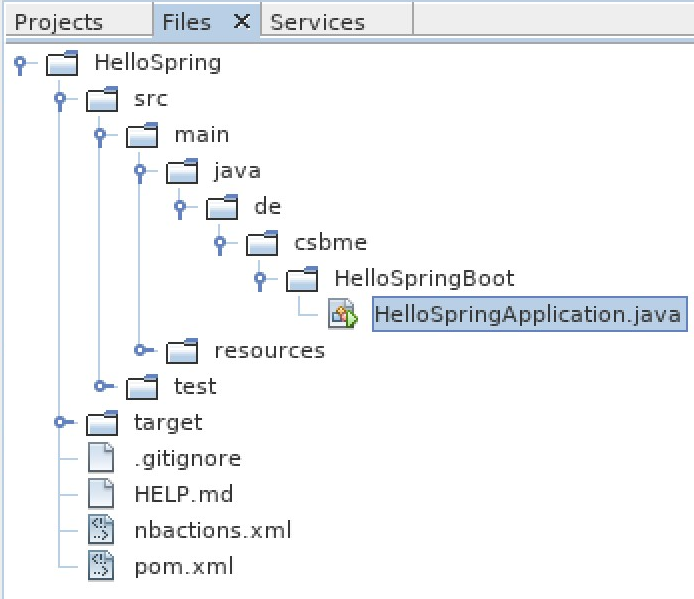
\includegraphics[width=5.5cm]{FirstProject/07_Dateistruktur}
}
&
\raisebox{\ht\strutbox-\height}{
	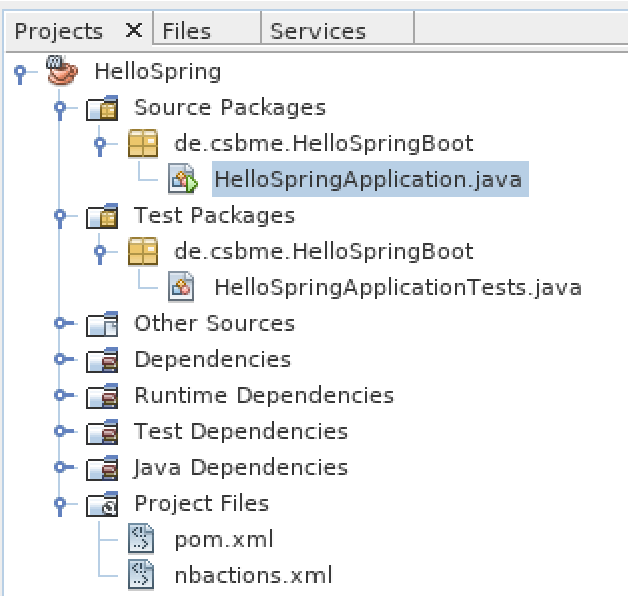
\includegraphics[width=5.5cm]{FirstProject/07_Projektstruktur}
}
\end{tabularx}

Die erstellten Dateien sehen etwa so aus:
\begin{lstlisting}[style=java] 
package de.csbme.HelloSpringBoot;

import org.springframework.boot.SpringApplication;
import org.springframework.boot.autoconfigure.SpringBootApplication;

@SpringBootApplication
public class HelloSpringApplication {
	
	public static void main(String[] args) {
		SpringApplication.run(HelloSpringApplication.class, args);
	}
	
}
\end{lstlisting}

Das Programm ist im Prinzip startbar - bleibt aber ohne jede Funktion. Für ein erstes "Hello World!" fehlen noch drei Anpassungen:
\\

Ein Import, der die nötigen Bibliotheken läd:
\begin{lstlisting}[style=java] 
import org.springframework.web.bind.annotation.*;
\end{lstlisting}

Die Annotation \textit{text@RestController}, die dem Framework mitteilt, dass diese Klasse regelt, wie auf HTTP-Request reagiert werden soll:
\begin{lstlisting}[style=java] 
@RestController
@SpringBootApplication
public class HelloSpringApplication {
\end{lstlisting}

Und eine Methode, die das Verhalten für den Fall festlegt, dass die Ressource "/" aufgerufen wird (also "localhost:8080/")
\begin{lstlisting}[style=java] 
@RequestMapping("/")
String home() {
	return "Hello World! \n";
}
\end{lstlisting}


Ein HTTP-GET-Request auf der Ressource "localhost:8080/" sollte jetzt ein "Hello World!" als Antwort erhalten.
In einem Linux/MacOSX-Terminal mit installiertem \texttt{curl} getestet:
\begin{lstlisting}[language=bash] 
$ curl localhost:8080
Hello World!
\end{lstlisting}
Oder unter Windows über die PowerShell (curl ist hier ein Alias des CmdLets Invoke-WebRequest)
\begin{lstlisting}[style=powershell] 
> Invoke-WebRequest http://localhost:8080/


StatusCode        : 200
StatusDescription :
Content           : Hello World!

RawContent        : HTTP/1.1 200
Content-Length: 14
Content-Type: text/plain;charset=UTF-8
Date: Sun, 22 Sep 2019 16:14:40 GMT

Hello World!

Forms             : {}
Headers           : {[Content-Length, 14], [Content-Type, text/plain;charset=UTF-8], [Date, Sun, 22 Sep 2019 16:14:40
	GMT]}
Images            : {}
InputFields       : {}
Links             : {}
ParsedHtml        : mshtml.HTMLDocumentClass
RawContentLength  : 14
\end{lstlisting}

Sofern der Port 8080 bereits für andere Dienste benötigt wird lässt sich dieser Default-Port überschreiben, z.B. in der Datei src/main/resources/application.properties
\begin{lstlisting}[style=java] 
server.port=8085
\end{lstlisting}

Check:
\begin{lstlisting}[language=bash] 
$ curl localhost:8085
Hello World!
\end{lstlisting}

\begin{lstlisting}[style=java] 
package de.csbme.HelloSpringBoot;

import org.junit.Test;
import org.junit.runner.RunWith;
import org.springframework.boot.test.context.SpringBootTest;
import org.springframework.test.context.junit4.SpringRunner;

@RunWith(SpringRunner.class)
@SpringBootTest
public class HelloSpringApplicationTests {
	
	@Test
	public void contextLoads() {
		
		
	}
	
}
\end{lstlisting}


\begin{lstlisting}[style=java] 
package de.csbme.HelloSpringBoot;

import org.junit.Test;
import org.junit.runner.RunWith;
import org.springframework.boot.test.context.SpringBootTest;
import org.springframework.test.context.junit4.SpringRunner;

import org.springframework.beans.factory.annotation.Autowired;
import org.springframework.boot.test.autoconfigure.web.servlet.AutoConfigureMockMvc;
import org.springframework.http.MediaType;
import org.springframework.test.web.servlet.MockMvc;
import org.springframework.test.web.servlet.request.MockMvcRequestBuilders;

@AutoConfigureMockMvc
@RunWith(SpringRunner.class)
@SpringBootTest
public class HelloSpringApplicationTests {
	
	@Autowired
	private MockMvc mvc;
	
	@Test
	public void contextLoads() {
		mvc.perform(MockMvcRequestBuilders.get("/"))
		.andExpect(status().isOk())
		.andExpect(content().string("Hello World! \n"));
	}
	
}

}
\end{lstlisting}

\begin{lstlisting}language=xml] 
<?xml version="1.0" encoding="UTF-8"?>
<project xmlns="http://maven.apache.org/POM/4.0.0" xmlns:xsi="http://www.w3.org/2001/XMLSchema-instance"
xsi:schemaLocation="http://maven.apache.org/POM/4.0.0 https://maven.apache.org/xsd/maven-4.0.0.xsd">
	<modelVersion>4.0.0</modelVersion>
	<parent>
		<groupId>org.springframework.boot</groupId>
		<artifactId>spring-boot-starter-parent</artifactId>
		<version>2.1.8.RELEASE</version>
		<relativePath/> <!-- lookup parent from repository -->
	</parent>
	<groupId>de.csbme</groupId>
	<artifactId>HelloSpringBoot</artifactId>
	<version>0.0.1-SNAPSHOT</version>
	<name>HelloSpring</name>
	<description>Trying to Say Hello to SpringBoot</description>

	<properties>
		<java.version>11</java.version>
	</properties>

	<dependencies>
		<dependency>
			<groupId>org.springframework.boot</groupId>
			<artifactId>spring-boot-starter-web</artifactId>
		</dependency>

		<dependency>
			<groupId>org.springframework.boot</groupId>
			<artifactId>spring-boot-starter-test</artifactId>
			<scope>test</scope>
		</dependency>
	</dependencies>

	<build>
		<plugins>
			<plugin>
				<groupId>org.springframework.boot</groupId>
				<artifactId>spring-boot-maven-plugin</artifactId>
			</plugin>
		</plugins>
	</build>
</project>
\end{lstlisting}

\end{document}
